
Die folgende Tabelle zeigt die Ergebnisse
der Optimierung der Testfunktionen
mit Variablenbeschr�nkung, wobei die Minimalstellen
immer noch in dem zul�ssigen Bereich bleiben.

\begin{table}[h]
\centering
\begin{tabular*}{0.5\linewidth}{@{\extracolsep{\fill}}lcc}
  \toprule
  Problem &   SSN   &   SQP   \\
  \cmidrule{2-3}
          & \multicolumn{2}{c}{T (ms)} \\
  \midrule
  Rosenbrock     &  16.72  &  25.62  \\
  Himmelblau     &  17.34  &  30.31  \\
  Bazaraa-Shetty &  53.59  & 109.38  \\
  Colville       & 593.75  & 656.25  \\
  \bottomrule
\end{tabular*}
\caption{Vergleich}
\end{table}

\begin{table}[h]
\centering
\begin{tabular*}{0.8\linewidth}{@{\extracolsep{\fill}}c|cccccccccc}
  %\toprule
  $x_i$ & 1 & 2 & 3 & 4 & 5 & 6 & 7 & 8 & 9 & 10 \\
  \midrule
  $y_i$ & $-\frac{1}{2}$ & $-2$ & $-3$ & $-3$ & $-\frac{5}{2}$
    & $-2$ & $-1$ & 1 & 3 & $\frac{11}{2}$ \\
  %\bottomrule
\end{tabular*}
\caption{Gegebene Punkte}
\end{table}

\begin{figure}[ht]
\centering
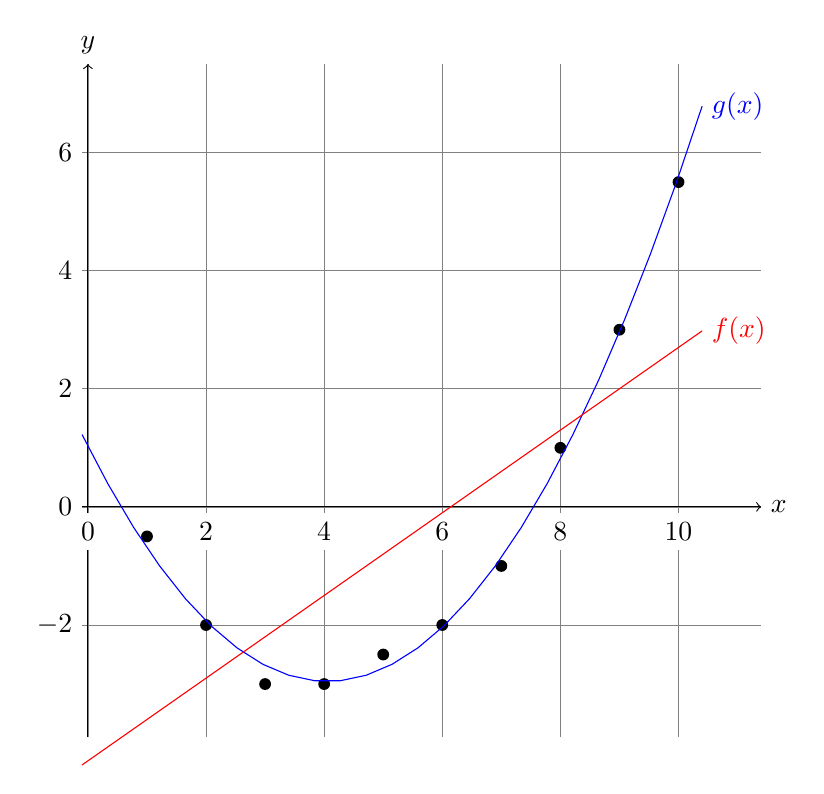
\begin{tikzpicture}[domain=-0.1:10.4,scale=0.75]
  \draw[very thin,color=gray,step=2] (-0.1,-3.9) grid (11.4,7.5);
  \draw[->] (-0.1,0) -- (11.4,0) node[right] {$x$};
  \draw[->] (0,-3.9) -- (0,7.5) node[above] {$y$};
  %\draw (-0.1,0.2) node [below left,fill=white] {0};
  \foreach \x in {0,2,4,...,10}
    \draw (\x,-0.1) node[below,fill=white] {$\x$};
  \foreach \y in {-2,0,2,4,6}
    \draw (-0.1,\y) node[left] {$\y$};
  \foreach \x/\y in
    {1/-0.5, 2/-2, 3/-3, 4/-3, 5/-2.5, 6/-2, 7/-1, 8/1, 9/3, 10/5.5}
    \fill (\x,\y) circle(0.1);
  \draw[color=blue] plot (\x,{0.242*(\x-4.056)^2-2.955}) node[right] {$g(x)$};
  \draw[color=red] plot (\x,{0.7*\x-4.3}) node[right] {$f(x)$};
\end{tikzpicture}
\caption{$f(x) = 0.7 x - 4.3
  \text{ und } g(x) = 0.242 (x - 4.056)^2 - 2.955$}
\end{figure}

Problem:
Finde den k�rzesten Abstand zwischen den Dreiecken $R$ und $S$
in der Abbildung~\ref{fig:abstand_zw_dreiecken}
und die zugeh�rigen Punkte $r^* \in R$ und $s^* \in S$, die
diesen k�rzesten Abstand bilden.

\begin{figure}[ht]
\centering
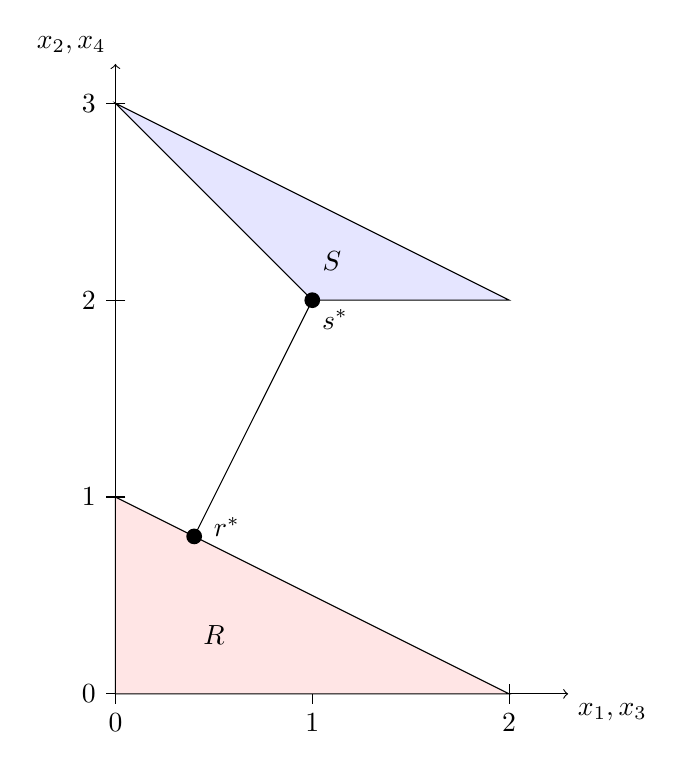
\begin{tikzpicture}[scale=2.5]
  \tikzstyle{information text}=[rounded corners,fill=yellow!10,inner sep=1ex]
  
  % Koordinatenachsen
  \draw[->] (0,0) -- (2.3,0) node [below right] {$x_1, x_3$};
  \foreach \x in {0,...,2}
    \draw (\x,0.05) -- (\x,-0.05) node [below] {\x};
  \draw[->] (0,0) -- (0,3.2) node [above left] {$x_2, x_4$};
  \foreach \y in {0,...,3}
    \draw (0.05,\y) -- (-0.05,\y) node [left] {\y};
  
  % Dreieck R
  \draw[fill=red!10] (0,0) -- (0,1) -- (2,0) -- cycle;
  \draw (0.5,0.3) node {$R$};
  
  % Dreieck S
  \draw[fill=blue!10] (0,3) -- (1,2) -- (2,2) -- cycle;
  \draw (1.1,2.2) node {$S$};
  
  % Punkt r*
  \fill (0.4,0.8) circle (0.04);
  \draw (0.45,0.85) node [right] {$r^*$};
  
  % Punkt s*
  \fill (1,2) circle (0.04);
  \draw (1,2) node [below right] {$s^*$};
  
  % Linie zwischen r* und s*
  \draw (0.4,0.8) -- (1,2);
  
\end{tikzpicture}
\caption{Dreieck}
\label{fig:abstand_zw_dreiecken}
\end{figure}
